\chapter{Complex Numbers}

\section{Intro}
In the following chapter these sources are used as background information \cite{complexpaul}, \cite{complexpurple}, \cite{complexnotebook}.
When simply using real numbers, you cannot always get the right answer to a given equation. An example of this could be the equation $x^2=-1$. Therefore sometimes we have to use complex numbers, which uses the imaginary unit $i$.
\begin{align*}
i=\sqrt{-1}.
\end{align*}
When squared, $i$ becomes:
\begin{align*}
i^2=-1,
\end{align*}
when cubed:
\begin{align*}
i^3=-i,
\end{align*}
and raised to the power of four:
\begin{align*}
i^4=1,
\end{align*}
These first four of $i$ creates a loop, $i$ to the fifth will, therefore, be the same as $i$ to the first, $i$ to the seventh is the same as $i$ to the third \\
Complex numbers have the form $z=a+ib$, where $z$ is the complex number that consists of an imaginary part and a real part. 
\begin{align*}
\text{Re}\{z\}=a
\\
\text{Im}\{z\}=b
\end{align*}
\\
An example of a complex numbers could be: $7+3i$, where 7 is the real part and 3 is the imaginary part. If $\text{Re}\{z\}=0$ the number is said to be pure imaginary. 
By using these complex numbers, infinitely more numbers can be created. 
%An example of this is the numbers: $2i$ and $-7i$, these are called pure imaginary numbers. When writing pure imaginary numbers you use the form $bi$, where $b$ is a real number that is not $0$. \\
%If you put another part on these imaginary numbers, thus $a+bi$ you get the complex numbers. Example $3+4i$ and $-12i+6$. In this case, $a$ is the real part and $b$, where $i$ is, is the imaginary part. $a$ and $b$ are real numbers. By using this method you can make all pure imaginary numbers into a complex number by writing it like this: $0+3i$. $3i$ does not stand alone anymore and is, therefore, a complex number now. You can also rewrite every real number into a complex by doing this $2+0i$. \\
%By using complex numbers you can, therefore, find a solution to any given polynomial equation. \\ 
Complex numbers are plotted on the complex plane. The complex plane consist of two axis, the real part and the imaginary part. An example of this is shown in the picture below.
\begin{figure}[H]
\centering
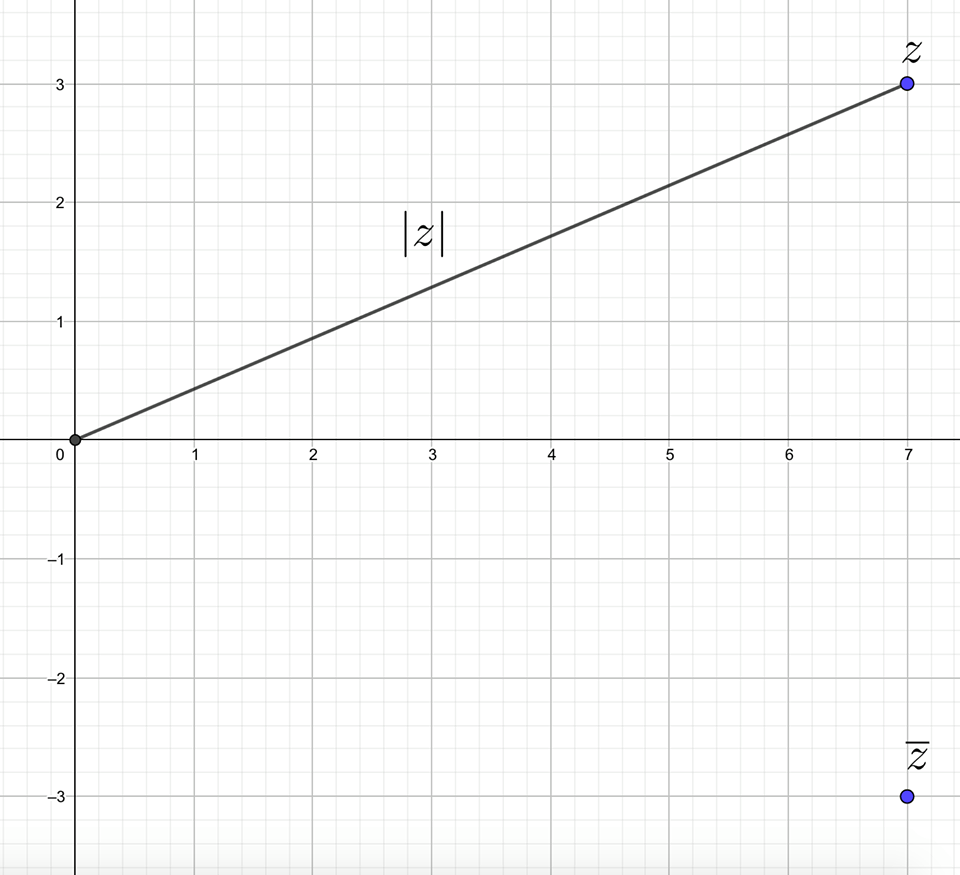
\includegraphics[scale=0.25]{fig/img/complex_plan}
\caption{The complex plane with the point $z=7+3i$}
\end{figure}
\noindent
The length from origin to the complex number is called modulus or absolute value of the number.
\begin{definition}{Modulus of a complex number}{}
The modulus of a complex number $z=a+ib$:
$$\mid z\mid=\sqrt{a^2+b^2}$$
\end{definition}
\noindent
To every complex number there also exists a complex conjugate. The conjugate of a complex number, has the same real part and opposite sign for the imaginary part.
\begin{definition}{Complex number conjugated}{}
The complex conjugate of $z=a+ib$ is given by:
$$\bar{z}=a-ib$$
\end{definition} 

\section{Adding and Subtracting}
When adding complex numbers the imaginary unit $i$, can be treated as a variable like in classic algebra. For instance, if you have something like $(5+2i)+(9+8i)$ then you can add the imaginary parts and the real parts and put it together on the general form; $a+bi$. In this case, we get $14+10i$. This rule can be explained in a general form: 
\begin{align*}
(a + bi) + (c + di) = (a + c) + i(b + d)
\end{align*}
Subtracting is similar because you can only subtract a imaginary part from another imaginary part, and the same goes for the constants. Here is an example:
\begin{align*}
(21 + 3i) - (2 - 2i) = 21 + 3i - 2 + 2i = 19 + 5i
\end{align*}
Similarly this can be put in a general form:
\begin{align*}
(a + bi) - (c + di) = (a - c) + i(b - d)
\end{align*}
From the examples above we can see that subtracting and adding with complex numbers is identical to subtracting and adding other and more familiar variables such as $x$, $y$ etc.

\section{Multiplying}
When multiplying with complex numbers it can get a little different than multiplying with other variables, as $i=\sqrt{-1}$ , $i^2=-1$ , $i^3=-i$ , $i^4=1$. \\
\begin{definition}{Multiplying complex numbers}{def:MCN}
The product of two complex numbers $z_1=a+ib$ and $z_2=c+id$ has the general form:
\begin{align*}
(a+ib)(c+id)&=a(c+di)+ib(c+di)
\\
&=ac+adi+bci+bdi^2
\\
&=(ac-bd)+i(ad+bc)
\end{align*}
\end{definition}
\begin{example}{Multiplying complex numbers}{}
Given two complex numbers $z_1=3+5i$ and $z_2=4-3i$ the product can found using \Cref{def:MCN}
\begin{align*}
(3+5i)(4-3i) = (3\cdot4-5\cdot(-3))+i(3\cdot(-3)+5\cdot4)=27+11i
\end{align*}
\end{example}


\section{Dividing}
When dividing with a complex number the aim is to get some values we can put on the general form $a + bi$. 
\begin{definition}{Dividing complex numbers}{def:DCM}
Division of two complex numbers where $z_1=a+ib$ and $z_2=c+id$ has the general form
\begin{align*}
\frac{a + bi}{c + di} 										
&= \frac{(a+bi)(c-di)}{(c+di)(c-di)} 						\\[1em]
&= \frac{a(c-di)+bi(c-di)}{a^2+b^2} 							\\[1em]
&= \frac{ac-adi+bci-bdi^2}{a^2+b^2}							\\[1em]
&= \frac{(ac+bd)+i(bc-ad)}{a^2+b^2}							\\[1em]
&= \frac{ac+bd}{a^2+b^2}+i \frac{bc-ad}{a^2+b^2}				
\end{align*}
\end{definition}
\begin{example}{Dividing complex numbers}{}
Given two complex numbers $z_1=18+10i$ and $z_2=3+2i$ can be found using \Cref{def:DCM}:
\begin{align*}
\frac{18 + 10i}{3 + 2i} &= \dfrac{18\cdot3+10\cdot2}{18^2+10^2}+i\dfrac{10\cdot3-18\cdot2}{18^2+10^2}
\\
&=\dfrac{37}{9}-\dfrac{1}{3}i
\end{align*}
\end{example}
From the example $\frac{37}{9} - \frac{1}{3}i$ is now on the form $a+ib$ with a and b being fractions. In the example the denominator is being conjugated and as a result of that the imaginary part of the denominator $ib$ disappears and is only left in the numerator. 
\section{Complex Numbers in Polar form}
Complex numbers in polar form is written on the form $(r,\theta)$, where $r$ is the distance from origin to the point $z$. $\theta$ is the angle from the real axis, when measured counter-clockwise. It will be negative if measured clockwise. \\
$r$ is also the modulus of $z$ and is therefore never negative $r=\mid z\mid$. $\theta$ is also an argument of z, this is written as $\theta=arg(z)$. %skal jeg have en forklaring på hvorfor det skal skrives på denne måde?
\\ 
The rectangular coordinates can be rewritten to polar coordinates. For this $a$ is expressed as $x=r\cdot \cos(\theta)$ and $bi$ is expressed as $bi=i\cdot r\cdot \sin(\theta)$. \\
$z$ is the expressed as:
$$z=r\cdot \cos(\theta) + i\cdot r\cdot \sin(\theta)$$
This can be rewritten as:
\begin{align}
z=r(\cos(\theta)+i \sin(\theta))
\end{align}
\begin{theorem}{Multiplication in polar form}{}
Given two complex numbers $z_1$ and $z_2$ where.
\begin{align*}
z_1=r_1(\cos(\theta_1)+i\sin(\theta_1)) 
\\
z_2=r_2(\cos(\theta_2)+i\sin(\theta_2))
\end{align*}
The multiplication of these are given by
\begin{align}
z_1 z_2=r_1r_2\left( \cos(\theta_1+\theta_2)+ i \sin(\theta_1+\theta_2)\right)
\end{align}
\end{theorem}
\begin{prof}{Multiplication in polar form}{}
\begin{align}
z_1 z_2&=r_1( \cos(\theta_1)+ i \sin(\theta_1))r_2( \cos(\theta_2)+ i \sin(\theta_2)) \nonumber
\\
\label{polar_multiplication}
z_1z_2&=r_1r_2\left( (\cos(\theta_1)\cos(\theta_2)-\sin(\theta_1) \sin(\theta_2))+i(\cos(\theta_1)\sin(\theta_2)+\sin(\theta_1)\cos(\theta_2)\right)
\end{align}
From trigonometry, sine of a sum and cosine of a sum can be expressed as:
\\
\begin{align} \label{sum_cos_sin}
\sin(\theta_1+\theta_2)=\cos(\theta_1)\sin(\theta_2)+\sin(\theta_1)\cos(\theta_2)
\\
\cos(\theta_1+\theta_2)=\cos(\theta_1)\cos(\theta_2)-\sin(\theta_1)\sin(\theta_1)
\end{align}
\\
These definitions are inserted in \eqref{polar_multiplication}.
\\
\begin{align}
z_1 z_2=r_1r_2\left( \cos(\theta_1+\theta_2)+ i \sin(\theta_1+\theta_2)\right)
\end{align}
\end{prof}
\section{The Complex Exponential Equation}
The complex exponential equation derives from Euler’s formula, and is necessary to explain the Laplace transformation. \\
%(noget mere tekst)

\begin{definition}{The complex exponential equation}{}
Given a complex number $z=a+ib$, $e^{z}$ is then defined as:
\begin{align*}
f(z)=e^z=e^ae^{ib}=e^a\cos(b)+i\sin(b)
\end{align*}
This function has the property:
$$\mid e^{a+ib} \mid = \mid e^a \mid$$
\end{definition}
\begin{theorem}{Multiplication of complex numbers in exponential form}{}
Given two complex numbers in exponential form $e^{z_1}$ and $e^{z_2}$ where:
\begin{align*}
z_1=a_1+ib_1
\\
z_1=a_2+ib_2
\end{align*}
The product of the two complex numbers is given by:
\begin{align}
e^{z_1}e^{z_2}=e^{z_1+z_2}
\end{align}
\end{theorem}
\begin{prof}{}{}
From definition 5.4 %skal ændres%
the product can be written as.
\begin{align*}
e^{z_1}e^{z_2}&=e^{a_1}(\cos(b_1)+i\sin(b_1))e^{a_2}(\cos(b_2)+i\sin(b_2))
\\
&=e^{a_1}e^{a_2}\left( (\cos(b_1)\cos(b_2)-\sin(b_1) \sin(b_2))+i(\cos(b_1)\sin(b_2)+\sin(b_1)\cos(b_2)\right)
\end{align*}
From \eqref{sum_cos_sin} this can be rewritten as:
\begin{align*}
&=e^{a_1}e^{a_2}(\cos(b_1+b_2)+i(\sin(b_1+b_2))
\end{align*}
Since both $e^{a_1}$ and $e^{a_2}$ are real numbers, their exponents can be added.
\begin{align*}
&=e^{a_1+a_2}(\cos(b_1+b_2)+i(\sin(b_1+b_2))
\end{align*}
From definition 5.4 %skal ændres
this can rewritten as:
\begin{align*}
&=e^{a_1+a_2}e^{i(b_1+b_2)}
\\
&=e^{a_1+ib_1}e^{a_2+ib_2}
\\
&=e^{z_1+z_2}
\end{align*} 
\end{prof}
\begin{theorem}{Differentiating a complex exponential function}{}
Given the complex function.
\begin{align}
f(z)=e^{z}=e^{a}(\cos(b)+i\sin(b))
\end{align}
Where $z=a+ib$. The differentiation of this function is given by:
\begin{align}
\dfrac{d}{dz}e^{z}=e^{z}
\end{align}
\end{theorem}
\begin{prof}{}{}
Given $z=a+ib$, the exponential function of this number is:
\begin{align}
f(z)=e^{z}=e^{a}(\cos(b)+i\sin(b))=e^{a}\cos(b)+e^{a}i\sin(b)
\end{align}
\end{prof}
\begin{prof}{}{proof:complex:diff:exp}
To show that the function $f(t)=e^{z t}$ is differentiable, where $z=a+ ib$:
\begin{align*}
	f(t) = e^{zt}= e^{(a+ib)t}= e^{at}  e^{ib t}.
\end{align*}
The imaginary part of the complex number $e^{ib\cdot t}$ can be rewritten using \cref{eulers_form}:
\begin{align*}
	f(t) =& e^{at}\big(\cos(bt)+i \cdot \sin(bt)\big), \\
		 =& e^{at}\cos(bt) + e^{at} i \cdot \sin(bt).
\end{align*}
The rewritten function can be differentiated using the chain rule:
\begin{align}
	\dfrac{d}{dt}f(t) =& ae^{at}\cos(bt) -ib \cdot \sin(bt)e^{at} + ia \cdot e^{at}\sin(bt) + ib \cdot e^{at}\cos(bt), \nonumber \\
	=& e^{at} \bigg( a\big(\cos(bt) + i \cdot \sin(bt)\big) + b\big(i \cdot \cos(bt) - \sin(bt)\big) \bigg), \nonumber \\
	=& e^{at}\bigg(a \cdot e^{ib \cdot t}+b\big(i \cdot \cos(bt) - \sin(bt)\big)\bigg), \nonumber \\
	=& a e^{t(a+ib)} + b e^{at}\big(i \cdot \cos(bt) - \sin(bt)\big). \label{proof:chain}
\end{align}
Since $i^2 = -1$, \eqref{proof:chain} can be rewritten. Furthermore, $a+ib$ is replaced with $z$:
\begin{align*}
	\dfrac{d}{dt}f(t) =& a e^{zt} + b e^{at}\big(i \cdot \cos(bt) + i^2 \cdot \sin(bt)\big).
\end{align*}
$i$ is now moved outside the parentheses, and \cref{eulers_form} is used to reduce the equation:
\begin{align*}
	\dfrac{d}{dt}f(t) =&  a e^{zt} + ib e^{at}\big(\cos(bt) + i \cdot \sin(bt)\big), \\
	=&  a e^{zt} + ib e^{at}e^{ib \cdot t}. \\
\end{align*}
Now $a+ib$ is replaced with $z$, and $e^{zt}$ can be placed outside of the parentheses:
\begin{align*}
	\dfrac{d}{dt}f(t) =&  a e^{zt} + ib e^{t(a+ib)}, \\
	=&  e^{zt}(a+ib).
\end{align*}
$a+ib$ is again replaced with $z$, and \cref{theorem:complex:exp} is proved.
\end{prof}

